\chapter{Ising model and complexity theory}


In this chapter, we will introduce the Ising spin--glass model and the related optimization problem
of finding its ground state. For this thesis, the model is of great importance, as instances of the said optimization problem serve as an input to quantum annealer, which we will describe in the next chapter.

To fully appreciate the potential usefulness of the quantum annealers, it is crucial to first discuss how hard finding the ground state of the Ising--spin glass is for the classical computer.
This will be discussed as the next point in the chapter, along with a brief introduction to complexity theory.

As the last point in this chapter, we will briefly introduce some commonly used heuristic methods for solving Ising optimization problems. Those, classical, heuristic methods, will serve as a baseline for comparison with quantum annealing and a recent tensor--network based approach discussed
later in the thesis.

\section{Ising model}
Consider a simple, undirected graph $G = (V, E)$ with $N$ nodes labelled by consecutive natural numbers. With each node $i \in V$ we associate a dichotomous spin variable $s_i \in \{-1, 1\}$. To each edge $\{i, j\} \in E$, we assign an interaction strength $J_{ij}$ and to each node $i \in V$ we assign local magnetic field $h_i$. Here, all $J_{ij}$ and $h_i$ are real numbers. For such a system, one can define the following energy function (Hamiltonian)
\begin{equation}
\label{eq:ising-hamiltonian}
H(\mathbf{s}) = \sum_{\langle i, j \rangle} J_{ij} s_i s_j +  \sum_{i=1}^N h_i s_i,
\end{equation}
where $\mathbf{s} = (s_i, \ldots, s_N)$ and the first sum runs over all edges in $E$\footnote{In the literature, the Ising Hamiltonian \eqref{eq:ising-hamiltonian} is often negated. However, the definition provided here is consistent with the one used by D-Wave, and thus more suitable for use in this thesis}.
\begin{figure}
    \centering
    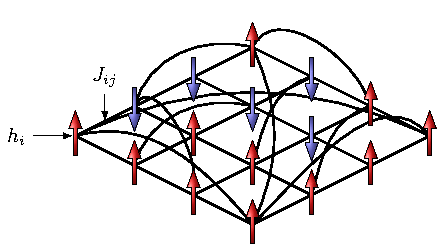
\includegraphics{figures/spins.pdf}
    \caption{An example of Ising spin--glass defined on the graph with $N=16$ nodes. Here, $h_i$ is a real number associated with $i$-th node, and $J_{ij}$ denotes coupling strength associated with an edge between $i$-th and $j$-th node. The configuration of each spin is marked by a red arrow pointing upwards (+1) or a blue arrow pointing downwards (-1).}
    \label{fig:my_label}
\end{figure}
For fixed model coefficients, one is typically interested in finding its \emph{ground state}, a configuration $\mathbf{s}$ that minimizes $H$. More generally, it might be desirable to search for $k \ll 2^N$ configurations with the lowest energy, the so-called \emph{low--energy spectrum}.

The model was introduced in 1920 by Wilhelm Lenz \cite{lenz} as a description of ferromagnetism in solids but is named after his student Ernst Ising, who studied and solved it in a one-dimensional case \cite{ising}. Despite the simple formulation, the problem of finding a ground state of Ising spin--glass is computationally hard \cite{barahoma}. Before expanding on this idea, let us first introduce the hierarchy of complexity classes.

\section{Algorithms and complexity}
Solving the computational problem requires suitable \emph{algorithm}, a description of steps to be performed by a computer to obtain a solution. It is hardly surprising that some problems might be solved in more than one way, i.e. there might exist different algorithms performing essentially the same task. Different algorithms solving the same problems might vastly differ in their demand on various resources, like memory or time needed to execute them. In practice, execution time (and usage of other resources) of a given algorithm might also vary between its implementations, depending on factors like programming language or libraries used and the hardware it is executed on. Therefore, measuring execution time is not that useful in characterizing the algorithm's performance.  Instead, it is more useful to characterize algorithms based on how their execution time scales (asymptotically) with increasing problem size. For instance, given an algorithm with execution time roughly proportional to the input size $N$, one might suspect that for problem instances large enough, it will perform better than the one with execution time proportional to $N^{2}$. This characteristic, known as computational complexity\footnote{Note that here we focus only on \emph{time complexity}, but other notions like memory complexity can be defined similarly}, is formalized by a big-$O$ notation (see appendix for more detailed description). Using this notation, the algorithms from the above example would be classified as $O(N)$ and $O(N^{2})$ respectively.

\section{Complexity classes}
Although there might exist multiple algorithms for solving a given computational problem, one might consider the minimal time complexity required to do so. More generally, one might group computational problems based on their demand on resources (in some fixed models of computation). In this view, sets of similar problems are called \emph{complexity classes}. The definition of some complexity classes might also be restricted to specific types of problems. For instance, one might consider only decision problems, i.e. problems to which the answer is yes or no.

One of the fundamental complexity classes is \textbf{P}, a class of decision problems solvable in polynomial time on a deterministic Turing Machine  \cite{arora}. Another class, \textbf{NP}, comprises all decision problems whose solution can be verified in polynomial time using a deterministic Turing Machine \cite{arora}.
One can immediately see that \textbf{P} $\subset$ \textbf{NP}. Indeed, if a problem is solvable in polynomial time, then it is also trivially verifiable in polynomial time. However, it is not immediately obvious if the inclusion is strict, and the question whether \textbf{P} $\ne$ \textbf{NP} is one of the most important, yet unsolved problems in theoretical computer science \cite{fortnow}.
The class of \textbf{NP--hard} problems comprises all the problems that are at least as hard as every problem in \textbf{NP}. More formally, given problem P is \textbf{NP--hard} if and only if solving every problem in \textbf{NP} can be reduced to solving P and then transforming the solution via some polynomial algorithm. Note that contrary to \textbf{P} and \textbf{NP},  the definition of \textbf{NP--hard} is not restricted to decision problems. A particular subclass of \textbf{NP--hard} problems, is an intersection of \textbf{NP} and \textbf{NP--hard} \cite{arora}. Figure \ref{fig:complexity} shows relationship between the discussed complexity classes both under assumptions \textbf{P} = \textbf{NP} and \textbf{P} $\ne$ \textbf{NP}.

Problems in the complexity class \textbf{P} are often considered tractable, or efficiently solvable, whereas problems not in \textbf{P} are perceived as hard and computationally demanding. However, this statement, known as Cobham's thesis, is imprecise, as it does not take into account multiple factors, including constant terms in big-O notation, or degrees of the involved polynomials. One can easily see that problem requiring $N^{10^6}$ time belongs to \textbf{P}, yet might be unsolvable even for very modest input of size $N=2$. Nevertheless complexity classes

\begin{figure}
    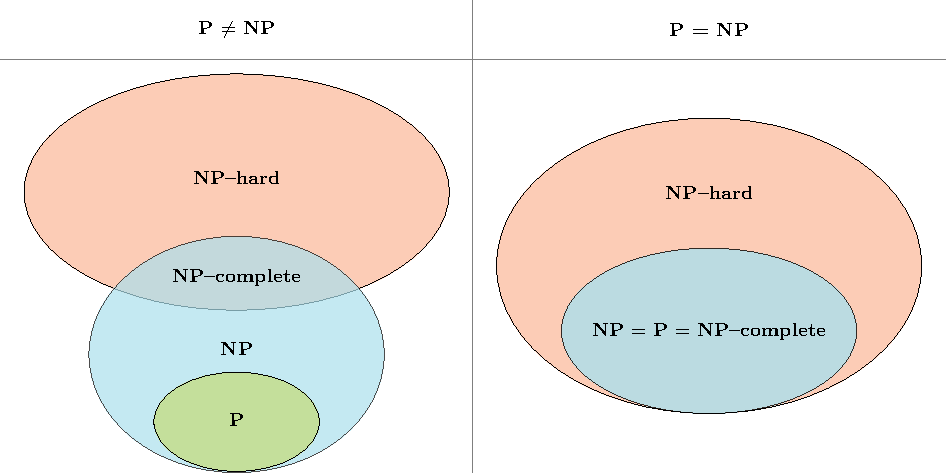
\includegraphics[width=\textwidth]{figures/complexity_new.pdf}
    \caption{Hierarchy of basic complexity classes. Under assumption of $\textbf{P} \ne \textbf{NP}$ (left), the hierarchy is richer and there exist problems in \textbf{NP}  that are not \textbf{NP}--complete. Under the opposite assumption (right), the hierarchy collapses. Notice that in both cases there exist \textbf{NP}--hard problems that are not in \textbf{NP}
    }
    \label{fig:complexity}
\end{figure}


\section{Ising model and complexity}

One can immediately see, that the state space of the Ising model with $N$ spins comprises $2^{N}$ different configurations. It might be tempting to reason that a problem with such an enormous number of possible solutions must be \textbf{NP--hard}. While this is indeed the case, the size of the solution space itself is not enough to reason about the problem's hardness\footnote{For instance, number of possible spanning trees in the complete graph of $N$ vertices is $N^{(N-2)}$, yet the minimum spanning tree problem is solvable in polynomial time via several algorithms \cite{clrs}}.
It was shown that finding a ground state of the Ising spin--glass in the case of three-dimensional lattices, as well as for some planar graphs,  is \textbf{NP--hard} \cite{barahoma}. The decision version of the problem (i.e. deciding whether the ground state has negative energy) is \textbf{NP--complete}. Multiple known \textbf{NP--hard} problems are reducible to finding the ground state of Ising spin-glass \cite{lucas}.

\section{Algorithms for solving Ising model}

As is the case with many \textbf{NP--hard} problems, there are many heuristic approaches for solving the Ising model. One family of such algorithms relies on Metropolis-Hastings \cite{beichl} algorithm for sampling from underlying Boltzmann distribution. In simulated annealing \cite{cook}, one lowers the temperature over time. Thus, the chance of accepting a locally worse solution is greater at the start of the algorithm and decreases with each iteration, which helps avoid getting stuck in a local minimum. In another approach from the same family, \emph{parallel tempering}, one simulates several replicas of the system, each of them in a different temperature. Neighboring replicas are allowed to exchange states, with exchange probability depending on their energy and temperature difference. Replicas with higher temperatures explore state space rapidly (thus reseeding the algorithm), while ones with lower temperatures refine the best solutions found so far. Various modifications of the aforementioned algorithms exist. For instance, one could employ isoenergetic cluster moves \cite{zhu} or adaptive choosing the number of sweeps performed between replica exchanges \cite{bittner}. Population annealing is another Monte Carlo method sharing similarities with simulated annealing and parallel tempering \cite{wang}. Other approaches for solving Ising spin--glasses include methods involving branch--and--bound framework \cite{rendl}, its chordal extensions \cite{baccari} or methods based on simulating dynamical systems \cite{sheldon}.

%%% Local Variables:
%%% mode: latex
%%% TeX-master: "../main"
%%% End:
